% Cross-Attention Fusion architecture schematic (figure 1).
% Build:  pdflatex architecture.tex   then   dvisvgm --pdf architecture.pdf
\documentclass[border=6pt]{standalone}
% Shared TikZ palette + primitive styles for the paper-style schematics.
% \input-ed by architecture.tex and training.tex. Colours ported from the old
% figures/toolkit.py PALETTE / EDGE / BAND_TINT.
\usepackage{tikz}
\usepackage{amsmath,amssymb,bm}
\usetikzlibrary{arrows.meta,positioning,fit,backgrounds,shadows.blur,calc}

% --- palette ---------------------------------------------------------------
\definecolor{ink}{HTML}{2B2B35}
\definecolor{muted}{HTML}{6B6B78}
\definecolor{line}{HTML}{9AA0AD}

\definecolor{clipFill}{HTML}{DBE7F5}\definecolor{clipEdge}{HTML}{7FA8D4}\definecolor{clipTint}{HTML}{EEF4FB}
\definecolor{queryFill}{HTML}{F5E6CC}\definecolor{queryEdge}{HTML}{D8B878}\definecolor{queryTint}{HTML}{FBF4E6}
\definecolor{trainFill}{HTML}{CDEACD}\definecolor{trainEdge}{HTML}{85C285}\definecolor{trainTint}{HTML}{EEF7EE}
\definecolor{negFill}{HTML}{F3D6D6}\definecolor{negEdge}{HTML}{DD9B9B}\definecolor{negTint}{HTML}{FCEEEE}
\definecolor{fuseFill}{HTML}{E8D6F3}\definecolor{fuseEdge}{HTML}{C298D8}\definecolor{fuseTint}{HTML}{F6EEFB}

\definecolor{posFill}{HTML}{D9EFD9}\definecolor{posEdge}{HTML}{5FAE5F}\definecolor{posInk}{HTML}{235C23}
\definecolor{negPillFill}{HTML}{F6D9D9}\definecolor{negPillEdge}{HTML}{D98989}\definecolor{negPillInk}{HTML}{7A2B2B}
\definecolor{goodGreen}{HTML}{2E7D32}
\definecolor{badRed}{HTML}{B3322F}
\definecolor{frostBlue}{HTML}{3D7CC0}
\definecolor{emberOrange}{HTML}{E8772E}
\definecolor{biton}{HTML}{7FA8D4}
\definecolor{bitflip}{HTML}{E0A52E}
\definecolor{avatarTile}{HTML}{F3F1EE}
\definecolor{avatarSil}{HTML}{B9BCC4}
\definecolor{badgeOk}{HTML}{2E9E4F}
\definecolor{badgeNo}{HTML}{CF4F4F}

% --- base styles -----------------------------------------------------------
\tikzset{
  every node/.style={font=\sffamily,text=ink},
  >={Stealth[round]},
  % rounded panel with soft shadow; role colours set via fill=...Fill, draw=...Edge
  panel/.style={rounded corners=4pt,draw,line width=0.9pt,blur shadow={shadow blur steps=5,
                shadow xshift=1.2pt,shadow yshift=-1.2pt,shadow opacity=28}},
  clip/.style ={panel,fill=clipFill, draw=clipEdge},
  query/.style={panel,fill=queryFill,draw=queryEdge},
  train/.style={panel,fill=trainFill,draw=trainEdge},
  neg/.style  ={panel,fill=negFill,  draw=negEdge},
  fuse/.style ={panel,fill=fuseFill, draw=fuseEdge},
  % a titled block: #1 = role style; use \blk macro below for title+subtitle text
  blk/.style 2 args={#1,align=center,inner sep=5pt},
  % stage band: dashed tinted backdrop drawn on the background layer
  band/.style={rounded corners=6pt,draw,line width=0.8pt,dash pattern=on 4pt off 3pt,
               inner sep=10pt},
  bandclip/.style ={band,fill=clipTint, draw=clipEdge},
  bandquery/.style={band,fill=queryTint,draw=queryEdge},
  bandtrain/.style={band,fill=trainTint,draw=trainEdge},
  bandneg/.style  ={band,fill=negTint,  draw=negEdge},
  bandfuse/.style ={band,fill=fuseTint, draw=fuseEdge},
  % signed pills
  pillpos/.style={rounded corners=7pt,fill=posFill,draw=posEdge,line width=0.9pt,
                  text=posInk,font=\sffamily\bfseries\small,inner sep=4pt},
  pillneg/.style={rounded corners=7pt,fill=negPillFill,draw=negPillEdge,line width=0.9pt,
                  text=negPillInk,font=\sffamily\bfseries\small,inner sep=4pt},
  % wires
  wire/.style={->,line width=1.1pt,ink},
  skipwire/.style={->,line width=1.0pt,muted,dash pattern=on 4pt off 3pt},
  % attribute-grid cells
  bitoff/.style={draw=line,line width=0.6pt,fill=white,minimum size=6pt,inner sep=0pt},
  biton/.style ={draw=line,line width=0.6pt,fill=biton,minimum size=6pt,inner sep=0pt},
  bitflip/.style={draw=bitflip,line width=1.5pt,minimum size=6pt,inner sep=0pt},
  wiretag/.style={font=\sffamily\scriptsize,text=muted,fill=white,inner sep=1.5pt,
                  fill opacity=0.85,text opacity=1},
  % --- layer-level (AlexNet/GoogLeNet-style) primitives ---
  lyr/.style={rounded corners=3pt,draw,line width=0.9pt,align=center,inner sep=4pt,
              font=\sffamily\small,fill=white,minimum height=0.78cm,minimum width=2.2cm},
  clipL/.style ={lyr,fill=clipFill, draw=clipEdge},
  queryL/.style={lyr,fill=queryFill,draw=queryEdge},
  trainL/.style={lyr,fill=trainFill,draw=trainEdge},
  negL/.style  ={lyr,fill=negFill,  draw=negEdge},
  fuseL/.style ={lyr,fill=fuseFill, draw=fuseEdge},
  % small elementwise-op node (\opn{$\oplus$})
  opn/.style={circle,draw=ink,line width=0.8pt,inner sep=0.5pt,font=\footnotesize,
              fill=white,minimum size=0.42cm},
  flow/.style={->,line width=1.0pt,ink},
}
% shape tag appended under a layer title: Title\dm{(B, 512)}
\newcommand{\dm}[1]{\\[1.5pt]{\ttfamily\scriptsize\color{muted}#1}}

% titled block: \blkbox{name}{role}{x,y}{width}{Title}{subtitle}
\newcommand{\blkbox}[6]{%
  \node[#2,minimum width=#4,align=center,inner sep=4pt] (#1) at (#3)
       {{\bfseries\small #5}\\[1pt]{\scriptsize\color{muted}#6}};}

% legend swatch
\newcommand{\swatch}[2]{\tikz[baseline=-0.5ex]\node[rounded corners=2pt,fill=#1,
  minimum width=9pt,minimum height=9pt,inner sep=0pt]{};~{\scriptsize #2}}

% placeholder face thumbnail: \avatar{name}{cx}{cy}{half-size}{edge colour}
\newcommand{\avatar}[5]{%
  \draw[rounded corners=2.5pt,fill=avatarTile,draw=#5,line width=1.1pt]
       (#2-#4,#3-#4) rectangle (#2+#4,#3+#4);
  \coordinate (#1) at (#2,#3);
  \begin{scope}
    \clip[rounded corners=2.5pt] (#2-#4,#3-#4) rectangle (#2+#4,#3+#4);
    \fill[avatarSil] (#2,#3+0.30*#4) circle ({0.55*#4});
    \fill[avatarSil] (#2,#3-0.55*#4) ellipse ({0.95*#4} and {0.72*#4});
  \end{scope}}
% pass/fail badge on the top-right of an avatar: \badge{cx}{cy}{half-size}{ok|no}
\newcommand{\badge}[4]{%
  \edef\bcol{\ifnum\pdfstrcmp{#4}{ok}=0 badgeOk\else badgeNo\fi}%
  \edef\bsym{\ifnum\pdfstrcmp{#4}{ok}=0 \noexpand\checkmark\else $\noexpand\times$\fi}%
  \draw[fill=\bcol,draw=white,line width=1.2pt] (#1+0.7*#3,#2+0.7*#3) circle ({0.42*#3});
  \node[text=white,font=\sffamily\bfseries\tiny] at (#1+0.7*#3,#2+0.7*#3) {\bsym};}

% 24-bit attribute grid (8 cols): \bitgrid{x}{y}{bit-string}{flip-list}
% bit-string: comma list of 0/1 (length 24); flip-list: comma indices (1-based) drawn highlighted
\newcommand{\bitgrid}[4]{%
  \begin{scope}[shift={(#1,#2)}]
    \foreach \bv [count=\i from 0] in {#3} {%
      \pgfmathtruncatemacro{\row}{div(\i,8)}\pgfmathtruncatemacro{\col}{mod(\i,8)}%
      \ifnum\bv=1\relax
        \node[biton]  (bc\i) at (0.24*\col,-0.24*\row) {};%
      \else
        \node[bitoff] (bc\i) at (0.24*\col,-0.24*\row) {};%
      \fi}%
    \edef\tmpflip{#4}%
    \ifx\tmpflip\empty\else
      \foreach \f in {#4} {\pgfmathtruncatemacro{\j}{\f-1}\node[bitflip] at (bc\j) {};}%
    \fi
  \end{scope}}

\begin{document}
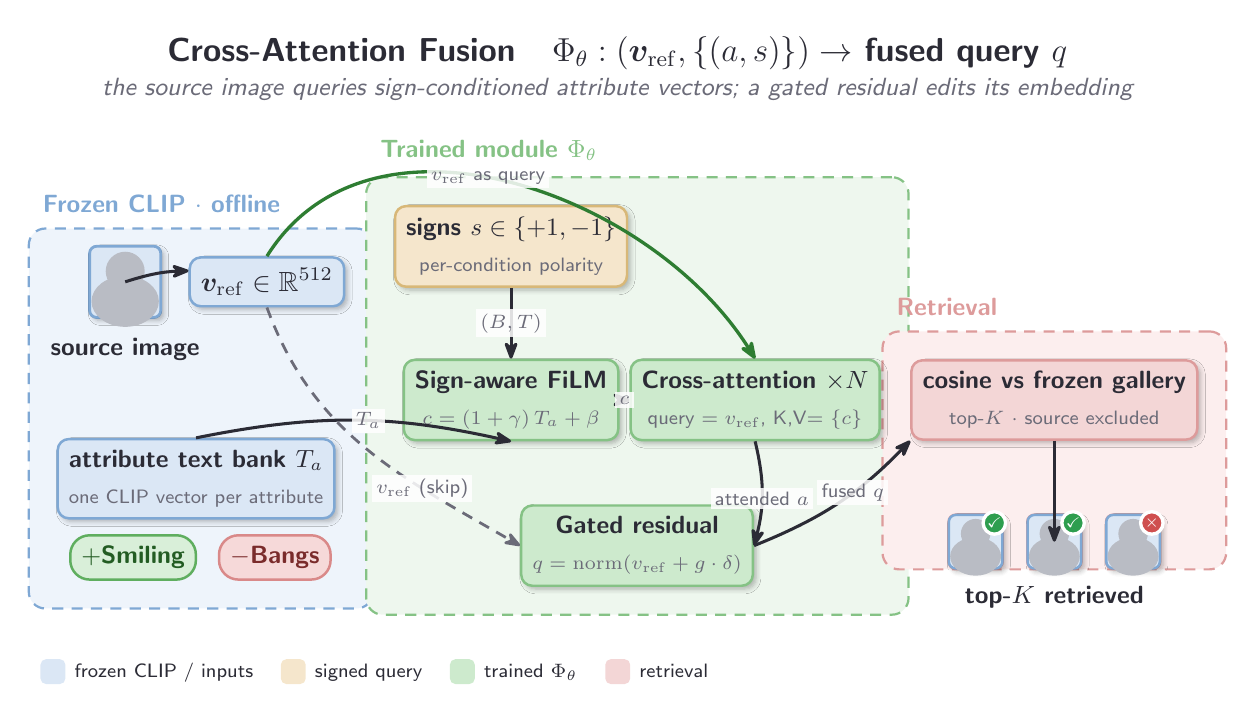
\begin{tikzpicture}[x=1cm,y=1cm]

  % ---- title ----
  \node[font=\sffamily\bfseries\large] at (7.75,8.3)
    {Cross-Attention Fusion\quad$\Phi_\theta:(\bm{v}_{\mathrm{ref}},\{(a,s)\})\to$ fused query $q$};
  \node[font=\sffamily\itshape\small,text=muted] at (7.75,7.85)
    {the source image queries sign-conditioned attribute vectors; a gated residual edits its embedding};

  % ================= band A : frozen CLIP inputs =================
  \avatar{src}{1.5}{5.4}{0.45}{clipEdge}
  \node[font=\sffamily\small\bfseries] at (1.5,4.55) {source image};
  \node[clip,inner sep=4pt] (vref) at (3.3,5.4) {$\bm{v}_{\mathrm{ref}}\in\mathbb{R}^{512}$};
  \draw[wire] (src) to[bend left=8] (vref);

  \blkbox{tbank}{clip}{2.4,2.9}{3.3cm}{attribute text bank $T_a$}{one CLIP vector per attribute}
  \node[pillpos] (pA) at (1.6,1.9) {$+$Smiling};
  \node[pillneg] (pB) at (3.4,1.9) {$-$Bangs};

  % ================= band B : trained module =================
  \blkbox{sgn}{query}{6.4,5.85}{2.6cm}{signs $s\in\{+1,-1\}$}{per-condition polarity}
  \blkbox{film}{train}{6.4,3.9}{2.6cm}{Sign-aware FiLM}{$c=(1+\gamma)\,T_a+\beta$}
  \blkbox{xatt}{train}{9.5,3.9}{2.7cm}{Cross-attention $\times N$}{query $=v_{\mathrm{ref}}$, K,V$=\{c\}$}
  \blkbox{gate}{train}{8.0,2.05}{2.9cm}{Gated residual}{$q=\mathrm{norm}(v_{\mathrm{ref}}+g\cdot\delta)$}

  % ================= band C : retrieval =================
  \blkbox{cos}{neg}{13.3,3.9}{3.4cm}{cosine vs frozen gallery}{top-$K$ $\cdot$ source excluded}
  \avatar{r1}{12.3}{2.1}{0.34}{negEdge}\badge{12.3}{2.1}{0.34}{ok}
  \avatar{r2}{13.3}{2.1}{0.34}{negEdge}\badge{13.3}{2.1}{0.34}{ok}
  \avatar{r3}{14.3}{2.1}{0.34}{negEdge}\badge{14.3}{2.1}{0.34}{no}
  \node[font=\sffamily\small\bfseries] at (13.3,1.4) {top-$K$ retrieved};

  % ---- wires ----
  \draw[wire] (tbank.north) to[bend left=12] node[wiretag,pos=0.55]{$T_a$} (film.south);
  \draw[wire] (sgn) -- node[wiretag]{$(B,T)$} (film);
  \draw[wire] (film) -- node[wiretag]{$c$} (xatt);
  % v_ref is the cross-attention query token: route over the top to stay clear
  \draw[wire,goodGreen,line width=1.2pt] (vref.north) to[out=58,in=122]
        node[wiretag,pos=0.46]{$v_{\mathrm{ref}}$ as query} (xatt.north);
  \draw[wire] (xatt.south) to[bend left=14] node[wiretag,pos=0.55]{attended $a$} (gate.east);
  \draw[skipwire] (vref.south) to[out=-70,in=150]
        node[wiretag,text=muted,pos=0.7]{$v_{\mathrm{ref}}$ (skip)} (gate.west);
  \draw[wire] (gate.east) to[bend right=12] node[wiretag,pos=0.6]{fused $q$} (cos.south west);
  \draw[wire] (cos.south) -- (r2.north);

  % ================= stage bands (background) =================
  \begin{scope}[on background layer]
    \node[bandclip, fit=(src)(vref)(tbank)(pA)(pB),
          label={[anchor=south west,font=\sffamily\bfseries\small,text=clipEdge,xshift=2pt,yshift=2pt]north west:Frozen CLIP $\cdot$ offline}] {};
    \node[bandtrain,fit=(sgn)(film)(xatt)(gate),
          label={[anchor=south west,font=\sffamily\bfseries\small,text=trainEdge,xshift=2pt,yshift=2pt]north west:Trained module $\Phi_\theta$}] {};
    \node[bandneg,  fit=(cos)(r1)(r3),
          label={[anchor=south west,font=\sffamily\bfseries\small,text=negEdge,xshift=2pt,yshift=2pt]north west:Retrieval}] {};
  \end{scope}

  % ================= legend =================
  \node[anchor=west,align=left,font=\sffamily] at (0.3,0.45)
    {\swatch{clipFill}{frozen CLIP / inputs}\quad\swatch{queryFill}{signed query}\quad
     \swatch{trainFill}{trained $\Phi_\theta$}\quad\swatch{negFill}{retrieval}};

\end{tikzpicture}
\end{document}
